\section{Perulangan Pada Python}
Perulangan dalam bahasa pemrograman berfungsi untuk memerintahkan komputer melakukan sesuatu secara berulang-ulang. Terdapat dua jenis perulangan dalam bahasa pemrograman python, yaitu perulangan dengan for dan while.
\subsection{While dan For}
Perulangan while disebut dengan uncounted loop (perulangan yang tak terhitung), sementara perulangan for disebut dengan counted loop (perulangan yang terhitung). Perbedaannya adalah ada statement while, biasanya memiliki ciri berupa pengecekan kondisi dan perulangan dilakukan diawal. Sedangkan pada statement for, memiliki ciri berupa inisialisasi perulangan dilakukan diawal statement dan perulangan tersebut akan berhenti ketika syarat/ kondisi yang telah ditentukan terpenuhi\cite{santoso2009bahasa}.

\subsection{Perintah Break, Continue dan Pass Perintah Break}
\subsubsection{Perintah Break}
Perintah break dipakai untuk menghentikan proses berjalannya iterasi atau perulangan pada statement for atau while\cite{arfian2012rekayasa}.Dan semua kode setelah pernyataan break akan segera diabaikan. Pernyataan break ini dapat kita gunakan pada pengulangan while dan for.
Statement yang berada di bawah break tidak akan di eksekusi dan program akan keluar dari proses looping.  
Contoh break : 
\begin{equation}
>>> x = 1     
>>> while x < 5:     
...    if x == 3:     
...      break     
...    print x     
...    x = x+1                                                                                                                    
... else:          
print "Loop sdh selesai dikrjkn"   
 ...     
1    
2 
\end{equation}

\subsubsection{Perintah Continue}
Perintah continue dapat dipakai untuk meloncati sebuah perulangan, maksudnya adalah intruksi yang seharusnya dapat dilewati, hal ini berarti instruksi tidak akan dijalankan\cite{arfian2012rekayasa}. pernyataan continue akan dilakukan pengulangan mulai dari awal lagi. Dan mengabaikan semua kode yang tersisa pada loop untuk menuju keawal loop lagi.
Misal:
\begin{equation}
for(int i = l; i <= 100; i++){
    if(i % 2 == 0){
        continue;
    }
    System.out.println(i);
    }
\end{equation}

Jika program tersebut dijalankan, maka hasilnya akan menampilkan angka-angka ganjil saja, hal ini disebabkan karena saat nilai i merupakan angka genap, maka statement continue akan membuat program tidak menampilkan angka genap.

\subsubsection{Perintah Pass}
Sebenarnya perintah pass tidak memiliki fungsi yang sangat penting. Dan bahkan sangat jarang digunakan oleh programmer. Jadi perintah pass ini sebenarnya hanya mengisi kekosongan saja, agar program tidak eror nantinya.perintah pass akan Menyebabkan program tidak melakukan tindakan. Digunakan untuk mengabaikan sesuatu statement perulangan, pengkodisian, class dan fungsi yang belum di definisikan badan programnya agar tidak terjadi error.
\begin{equation}
for i in range (5) :
    if i == 5 :
        pass
    print(i)
    \end{equation}

Jadi seperti yang sudah dikatakan sebelumnya, perintah pass ini memiliki fungsi untuk mengisi kekosongan dari sebuah penyeleksian ataupun perulangan.

 \subsubsection{Perintah return}
Perintah return dapat menghentikan suatu proses dari fungsi sebelum mengakhiri fungsi tersebut. Alasan menggunakan perintah return adalah jika menemui sebuah kesalahan kondisi, yang berarti nilai suatu fungsi tersebut mengembalikan nilai null (kosong) : 
import math
\begin{equation}
def print_log (x):
  if x <= 0 :
    print x, 
\"Bilangan lebih sama dengan 0\"  
  return  
hasil = math.log (x) 
 print \"Hasil log dari\", x, \"adalah\", hasil 
 \end{equation}
 
 Fungsi print_log() mengambil sebuah parameter x. Hal yang dilakukan pertama kali adalah memeriksa apakah nilai x lebih kecil atau sama dengan 0, yang dapat menghasilkan pesan kesalahan jika di proses dalam instruksi perintah selanjutnya maka diberi perintah return untuk keluar dari fungsi tersebut. Alur jalannya program segera dikembalikan ke pemanggil dari fungsi tersebut, dan instruksi - instruksi berikutnya tidak akan dijalankan. Perhatikan! untuk memanggil fungsi dari modul math harus menggunakan perintah import <nama-modul> .

 \subsubsection{Rekursif}

Telah disebutkan sebelumnya, bahwa kita dapat memanggil suatu fungsi di dalam fungsi lainnya, dan Anda telah melihat beberapa contoh - contohnya. Kita juga dapat memanggil fungsi itu sendiri yang kemudian di kenal dengan istilah rekursif. Mungkin sekilas hal itu tidak memberi alasan mengapa rekursif ini adalah hal yang baik, tetapi akan berubah menjadi program yang menarik.Sebagai contohnya, lihat 
fungsi berikut :

\begin{equation}
def hitung_mundur (x):

if x == 0 :

print "Sudah nol koq!"

else :

print x

hitung_mundur (x-1)
 \end{equation}
 
fungsi diatas menampilkan program hitung mundur dari nilai parameter x yang diberikan, parameter tersebut seharusnya sebuah bilangan integer yang positif, dan jika nilai x sama dengan 0 akan menampilkan string yang memberitahu bahwa nilai x adalah 0.Kalau tidak nol(0) maka akan memanggil fungsi itu sendiri dan memberi nilai x-1 sebagai parameternya.

Prosesnya adalah sebagai berikut, jika kita memanggil fungsi tersebut dengan nilai 3, maka nilai 3 akan di check apabila bukan nol (0) maka akan di cetak, dan memanggil fungsi itu sendiri dengan parameter 3-1, yaitu nilai 2, kemudian nilai 2 akan di periksa apakah nilai 2 sama dengan 0, jika bukan maka akan di cetak, dan memanggil fungsi tersebut dengan nilai parameter 1, di check kembali bila bukan
nol (0) maka akan akan memberikan parameter x-1 ke fungsi itu sendiri, setelah itu maka fungsi tersebut di beri paramater 0 maka string "Sudah nol koq!" dicetak, kemudian kembali lagi ke fungsi sebelumnya dengan nilai 1, kembali ke nilai 2,kembali ke nilai 3.
Jadi tampilan hasilnya akan seperti berikut.

3

2

1

Sudah nol koq!

Hal ini akan berbeda jika perintah print diletakkan setelah pemanggilan fungsi rekursif itu sendiri. Misalnya :
\begin{equation}
def hitung_maju(x):

if x == 0 :

print "Sudah nol, Mulai!"

else :

 \end{equation}
 \begin{equation}
hitung_maju (x-1)

print x

maka tampilannya akan menjadi :
 \end{equation}
Sudah nol, Mulai!

1

2

3

 

\subsection{Nested Loop}
Nested Loop (Perulangan Bertingkat) adalah semua tipe perulangan yang dapat dipakai di dalam perulangan yang lain. Jadi Perulangan for bisa dipakai di dalam for yang lain, perulangan for bisa berada didalam perulangan while, perulangan while bisa dipakai di dalam perulangan while yang lain, dan perulangan while bisa di dalam perulangan for.
\subsubsection{Contoh Penggunaan Nested Loop}
Format nested loop \(for di dalam for\)
\begin{equation}
For iterasi_var_1 in urutan_1:
	Statements_untuk_perulangan_for_yang_di_luar
...
For iterasi_var_1 in urutan_2:
	Statements_untuk_perulangan_for_yang_di_dalam
...
Statements_untuk_perulangan_for_yang_di_luar
...
\end{equation}

Format nested loop \(while di dalam while\)
\begin{equation}
While expressions:
	Statements_untuk_perulangan_while_yang_di_dalam
...
Statements_untuk_perulangan_whle_yang_di_luar
...
\end{equation}

Contoh :
\begin{equation}
X = int(input(“Masukkan jumlah bariss: “))
For i in range (x) :
	For j in range(i+1):
		Print(“*”, end=””)
	Print()
\end{equation}
Saat di Run Module maka :
Masukkan jumlah bariss: 5 \(inputkan 5\)
*
**
***
****
***** 
Muncul 5 baris isi bintang

\subsubsection{Nested Loop for Nested Data}
Disini kita memiliki list data dari murid-murid. Jadi, setiap murid memiliki nama yang dipasangkan dengan list subyek(mata pelajaran) yang mereka ambil. Dan akan mencetak setiap nama murid, dan jumlah dari subyek (mata pelajaran) yang mereka ambil
\begin{equation}
students = [
    ("John", ["TIK", "IPS"]),
    ("Vusi", ["Matematika", "TIK", "IPA"]),
    ("Jess", ["TIK", "Bahasa Indonesia", "Ekonomi", "Pendidikan Agama Islam"]),
    ("Sarah", ["Biologi", "Matematika", "Ekonomi", "Kimia"]),
    ("Zuki", ["Sosiologi", "Ekonomi", "Biologi", "Matematika", "Bahasa Inggris"])]

for (name, subjects) in students:
    print(name, "takes", len(subjects), "courses")
\end{equation}
Lalu, setelah dijalankan (run) maka akan tampil seperti ini:
John takes 2 courses
Vusi takes 3 courses
Jess takes 4 courses
Sarah takes 4 courses
Zuki takes 5 courses

\subsection{While Loop}
Perintah While pada pyton biasanya memiliki ciri berupa pengecekan kondisi dan perulangan dilakukan diawal\cite{santoso2009bahasa}. Alur prosesnya adalah ketika sebuah program dijalankan dan kemudian menemukan sebuah kondisi dimana menggunakan loop atau perulangan while, jika kondisi true maka statment itu akan dieksekusi kemudian akan di cek lagi kondisinya. Setelah selesai statmentnya masih true dieksekusi lalu akan mengecek lagi kondisinya dan terus seperti itu, dan jika false statementntya maka akan keluar dari perulangan dan akan melanjutkan ke program selanjutnya.

\subsection{Perulangan do-while}
Perulangan do-while merupakan perulangan yang  mirip dengan perulangan while namun perbedaannya\cite{arfian2012rekayasa}, pada perulangan do-whiile, maka minimal instruksi akan dijalnkan sekali. Contoh statement do-while:
\begin{equation}
int jumlah = 100;
do{
    System.out.println(jumlah);
    jumlah++; // naikkan jumlah
}while(jumlah <= 10);
\end{equation}
Jika program itu dijalankan, maka akan menghasilkan keluaran 100,  yang artinya walaupun kondisinya salah, namun minimal isi instruksi akan dijalankan sekali, hal ini disebabkan karena proses do-while berbeda dengan while,  yang dimana do-while pertama melakukan instruksi setelah itu baru mengecek kondisi, sedangkan while pertama mengecek kondisi baru melakukan instruksi. 

\subsection{Perulangan \(for loop\)}
FOR Loop dipakai untuk melakukan perulangan atau iterasi mencapai batas atau jarak yang telah ditentukan/cite{santoso2009bahasa}.

Kegunaan
\begin{enumerate}
\item Ketika ingin pergi ke item urutan tertentu seperti pada list atau string
\item Ketika ingin melakukan perulangan kode beberapa kali
\end{enumerate}
For interaksi_var in ururan
Statements
Print(“bukan bagian perulangan”) 

\subsection{For Loop}
Perulangan for disebut juga counted loop \(perulangan yang terhitung\)
Pengulangan for digunakan untuk pengulangan dengan muatan yang banyak\cite{van2007python}.
keistimewaan perulanga pada for adalah , perulangan dapat di hentikan pada saat kondisi tertentu. pada python, statemen for bekerja mengulang berbagai macam tipe data sekuensial seperti pada list, string dan tuple
Contohnya Seperti :
\begin{equation}
for a in range(0, 10):
	print a
\end{equation}
Hasil Outputnya :
\begin{equation}
python for.py
0
1
2
3
4
5
6
7
8
9
\end{equation}


\subsection{While Loop}
perulangan while disebut juga uncounted loop \(perulangan yang tak terhitung\)
Pengulangan while biasanya digunakan untuk sesuatu yang ga pasti.
Contohnya Seperti :
\begin{equation}
a = 0
while true:
	if a < 10:
		print "saat ini a bernilai: ", a
		a = a + 1
	else a >= 5:
		break
\end{equation}
Hasil Outputnya :
\begin{equation}
python while.py
saat ini a bernilai: 0
saat ini a bernilai: 1
saat ini a bernilai: 2
saat ini a bernilai: 3
\end{equation}

\subsection{For looping with list}
Contohnya Seperti :
\begin{equation}
hero_dota2_character = ["Mirana", "Axe", "Tusk"]
for character in hero_dota2_character:
	print character
\end{equation}
Hasil Outputnya :
\begin{equation}
python for-list.py
Mirana
Axe
Tusk
\end{equation}

\subsection{Infinite Loop}

Infine Loop adalah kondisi dimana program atau statement akan terus  mengeksekusi tanpa berhenti. Kondisi tersebut dapat dihentikan dengan menekan tombol CTRL+C.

Di bawah ini merupakan contoh program Infinite Loop :
\begin{equation}
# Nama file: inifinite_loop.py
# Program menampilkan tulisan Python tanpa henti

flag = 1

while (flag): print ("Python")
print ("Good bye!")
\end{equation}

\subsection{break and continue statements}
Jeda digunakan untuk for loop atau while loop, sedangkan terus digunakan untuk melewati blok saat ini, dan kembali ke pertanyaan for atau while.
Contoh pertama seperti :
\begin{equation}
count = 0
while True:
    print(count)
    count += 1
    if count >= 5:
        break
		\end{equation}
Output pertama :
\begin{equation}
python while.py
0
1
2
3
4
\end{equation}

\subsection{Perintah break, continue dan else}
 Perintah break sama seperti dalam bahasa C, yaitu keluar dari ruang lingkup yang paling kecil dari
kondisi for atau while.
Perintah continue sama  seperti dalam bahasa C, fungsinya untuk melanjutkan statement
berikutnya dalam kondisi perulangan.
Pada kondisi perulangan juga diperbolehkan untuk menggunakan kalimat perintah else, yang dijalankan saat kondisi perulangan for tidak memenuhi suatu kondisi atau jika kondisi tersebut mengalami error/false, tetapi bukan pada saat kondisi perulangan dihentikan dengan perintah break. Berikut adalah contohnya:
\ref{2_bce}

\begin{figure}[ht]
    \centerline{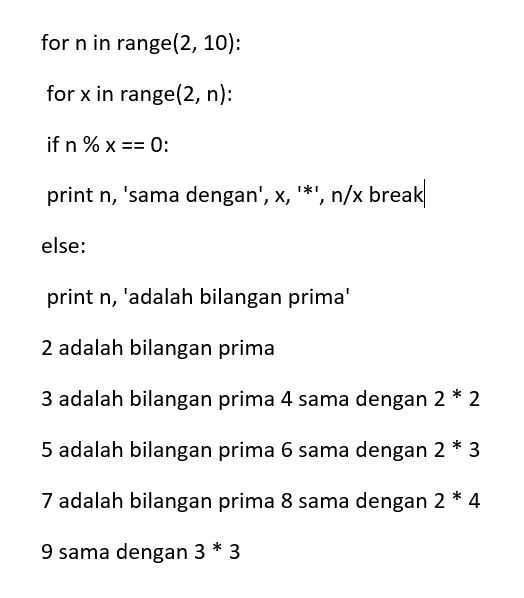
\includegraphics[width=1\textwidth]{figures/2_bce.JPG}}
    \caption{}
    \label{2_bce}
    \end{figure}

Penjelasannya adalah jika kondisi dalam perulangan for x in range\(2, n\) tidak terpenuhi maka alur perulangannya akan pindah ke ruang lingkup perintah else. 

\subsection{Range}
\subsubsection{Fungsi range\(\)}
Jika ingin melakukan perulangan dengan sejumlah yang diinginkan, fungsi built-in range sangat membantu. Fungsi tersebut menghasilkan sejumlah indeks dari nilai yang telah ditentukan. 
Contohnya :
\begin{equation}
>>> range(15)
[0, 1, 2, 3, 4, 5, 6, 7, 8, 9, 10, 11, 12, 13, 14]
Ataupun sebagian angka yang diinginkan. Contohnya :
>>> range (8, 15)
[8, 9, 10, 11, 12, 13, 14]
>>> range(0,9,3)
[0, 3, 6]
>>> range(0, 20, 3)
[0, 3, 6, 9, 12, 15, 18]
\end{equation}
 Contoh tersebut menunjukan kelipatan dari suatu interval bilangan yang mempunyai sintaks range\(<nilai-awal>, <nilai-akhir>, <kelipatan-angka>\).
\subsubsection{Contoh penggunaan range\(nilai_awal,nilai_akhir,pencacah\)}
Berikut ini contoh penggunaan range untuk menampilkan bilangan dari 1 – 100 dengan penambahan/pencacah 1 dengan menambahkan end=’ ’ agar bilangan tampil secara horizontal tidak pindah baris ke bawah
\begin{equation}
for i in range(1, 101, 1) :
    print(i, end=' ')
\end{equation}
Lalu, setelah perintah diatas dijalankan \(run\) maka akan tampil bilangan seperti berikut ini :
\ref{2_range}

\begin{figure}[ht]
    \centerline{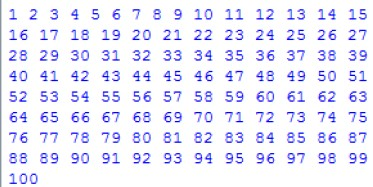
\includegraphics[width=1\textwidth]{figures/2_range.JPG}}
    \caption{hasil penggunaan range}
    \label{2_range}
    \end{figure}
    
\subsubsection{Contoh penggunaan range\(nilai_awal,nilai_akhir\)}
Berikut ini adalah contoh penggunaan range untuk menampilkan dari bilangan tertentu sampai bilangan tertentu dan menghitung banyaknya bilangan serta menghitung jumlah seluruh bilangan yang ada.
\begin{equation}
awal=int(input('Set Nilai Awal = '))
akhir=int(input('Set Nilai Akhir = '))

count=0
summ=0

print('Bilangan antara \%d dan \%d ' \%(awal,akhir))

for i in range(awal,akhir+1) :
	print(i, end=' ')
	count=count+1
	summ=summ+i

print('Bilangan di atas ada \%d bilangan' \%count)
print('Jumlah semua bilangan adalah \%d' \%summ)
\end{equation}

Setelah perintah diatas dijalankan \(run\) maka akan tampil bilangan seperti ini :
\ref{2_range2}

\begin{figure}[ht]
    \centerline{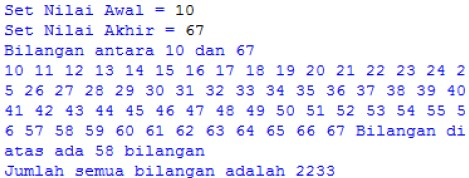
\includegraphics[width=1\textwidth]{figures/2_range2.JPG}}
    \caption{hasil penggunaan range}
    \label{2_range2}
    \end{figure}
    
\subsubsection{Contoh penggunaan range\(nilai_akhir\)}
Ini adalah contoh penggunaan range untuk menampilkan bilangan dari 0 – 100 dengan menambahkan end=’ ’ agar bilangan tampil secara horizontal tidak pindah baris ke bawah
\begin{equation}
for i in range(101):
	print(i,end=' ')
\end{equation}
Disini nilai akhir menggunakan operator < bukan ≤ jadi untuk menampilkan sampai angka 100 nilai akhir harus dibuat menjadi 101. Dan setelah perintah diatas dijalankan \(run\) maka akan tampil hasil seperti berikut ini :
\ref{2_range3}

\begin{figure}[ht]
    \centerline{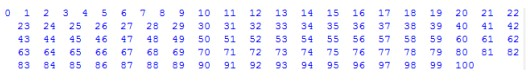
\includegraphics[width=1\textwidth]{figures/2_range3.JPG}}
    \caption{hasil penggunaan range}
    \label{2_range3}
    \end{figure}

\subsection{for loop with else}
For loop bisa memiliki blok else yang opsional juga. Bagian lain dijalankan jika item urutan digunakan dalam lingkaran for loop .
Pernyataan break bisa digunakan untuk menghentikan sebuah loop. Dalam kasus seperti itu, bagian yang lain diabaikan.

Oleh karena itu, bagian loop yang lain berjalan jika tidak terjadi pemutusan.

Berikut adalah contoh untuk menggambarkan hal ini.
\begin{equation}
script.py 
digits = [0, 1, 5]

for i in digits:
    print(i)
else:
    print("No items left.")
Output :
0
1
5
No items left.
\end{equation}

\subsection{Penggunaan loop dengan else statement}
Python mendukung untuk memiliki pernyataan lain yang terkait dengan pernyataan lingkaran

Jika else statement digunakan dengan for loop, pernyataan yang lain dijalankan saat loop telah habis mengulangi daftar.

Jika else statement digunakan dengan loop sementara, pernyataan yang lain dijalankan saat kondisinya menjadi salah.

\subsection{Middle-test loop}
Middle-test loop adalah sebuah perulangan yang akan mengeksekusi pada beberapa bagian body, kemudian akan melakukan pengujian exit berarti menguji dalam kondisi exit, lalu kemungkinan akan mengeksekusi beberapa bagian body lainnya. Disini dapat menggunakan while dan break secara bersama-sama. Terkadang kita membutuhkan looping dengan pengujian di tengah daripada pengujian di atas maupun di akhir.

\subsection{Penjelasan Penggunaan For Loop}
For loop secara tradisional digunakan saat Anda memiliki blok kode yang ingin Anda ulangi beberapa kali. Python untuk pernyataan iterates atas anggota urutan dalam urutan, mengeksekusi blok setiap waktu. Kontras untuk pernyataan dengan loop '' while '', digunakan bila suatu kondisi perlu diperiksa setiap iterasi, atau untuk mengulang blok kode selamanya.

\subsection{Pendukung kontrol dalam penggunaan looping python}
break berguna untuk menghentikan looping ketika terjadi kondisi tertentu.
continue berguna untuk melanjutkan sebuah operasi ketika pada blok statemen menghasilkan nilai yang diharapkan atau yang dicari.
pass kontrol ini tidak menghasilkan apapun dan pass akan berguna untuk mengecek apakah statemen berjalan apa tidak.
